\section{Implémentation}

Cette section présente de manière générale comment à été implémentée la structure de données, et motive les choix d'implémentation.

\subsection{Graphe de topologie}

Le réseau de dislocation peut s'apparenter à un graphe dont les nœuds et les segments portent des données. 

Le degré des nœuds d'un graphe représentant un réseau de dislocations est en général faible car il modélise des lignes, ce qui en fait un graphe discret. NuMoDis utilise cette notion de ligne en utilisant une représentation implicite du graphe qui liste les nœuds appartenant à une même ligne. Une telle implémentation permet de réduire l'empreinte mémoire mais n'est pas adaptée aux algorithmes parallèles.

La représentation du graphe est inspirée d'une implémentation orientée objet de graphe \footnote{Michael T. Goodrich et Roberto Tamassia, Algorithm Design: Foundations, Analysis, and Internet Examples, John Wiley \& Sons, 2002} en prenant soin de stocker les données des noeuds et des segments de manière contiguë afin d'être capable de les parcourir efficacement. 

Les nœuds et segments sont représentés par des objets contenant les données présentées en section \ref{sec:donnees_noeds_segments} en plus des informations sur la connectivité du graphe. Chaque nœud possède une liste des indices des segments qui lui sont incidents, et chaque segment contient les indices des deux nœuds connectés. La figure \ref{fig:representation_graphe} illustre cette représentation du graphe. 

\begin{figure}
	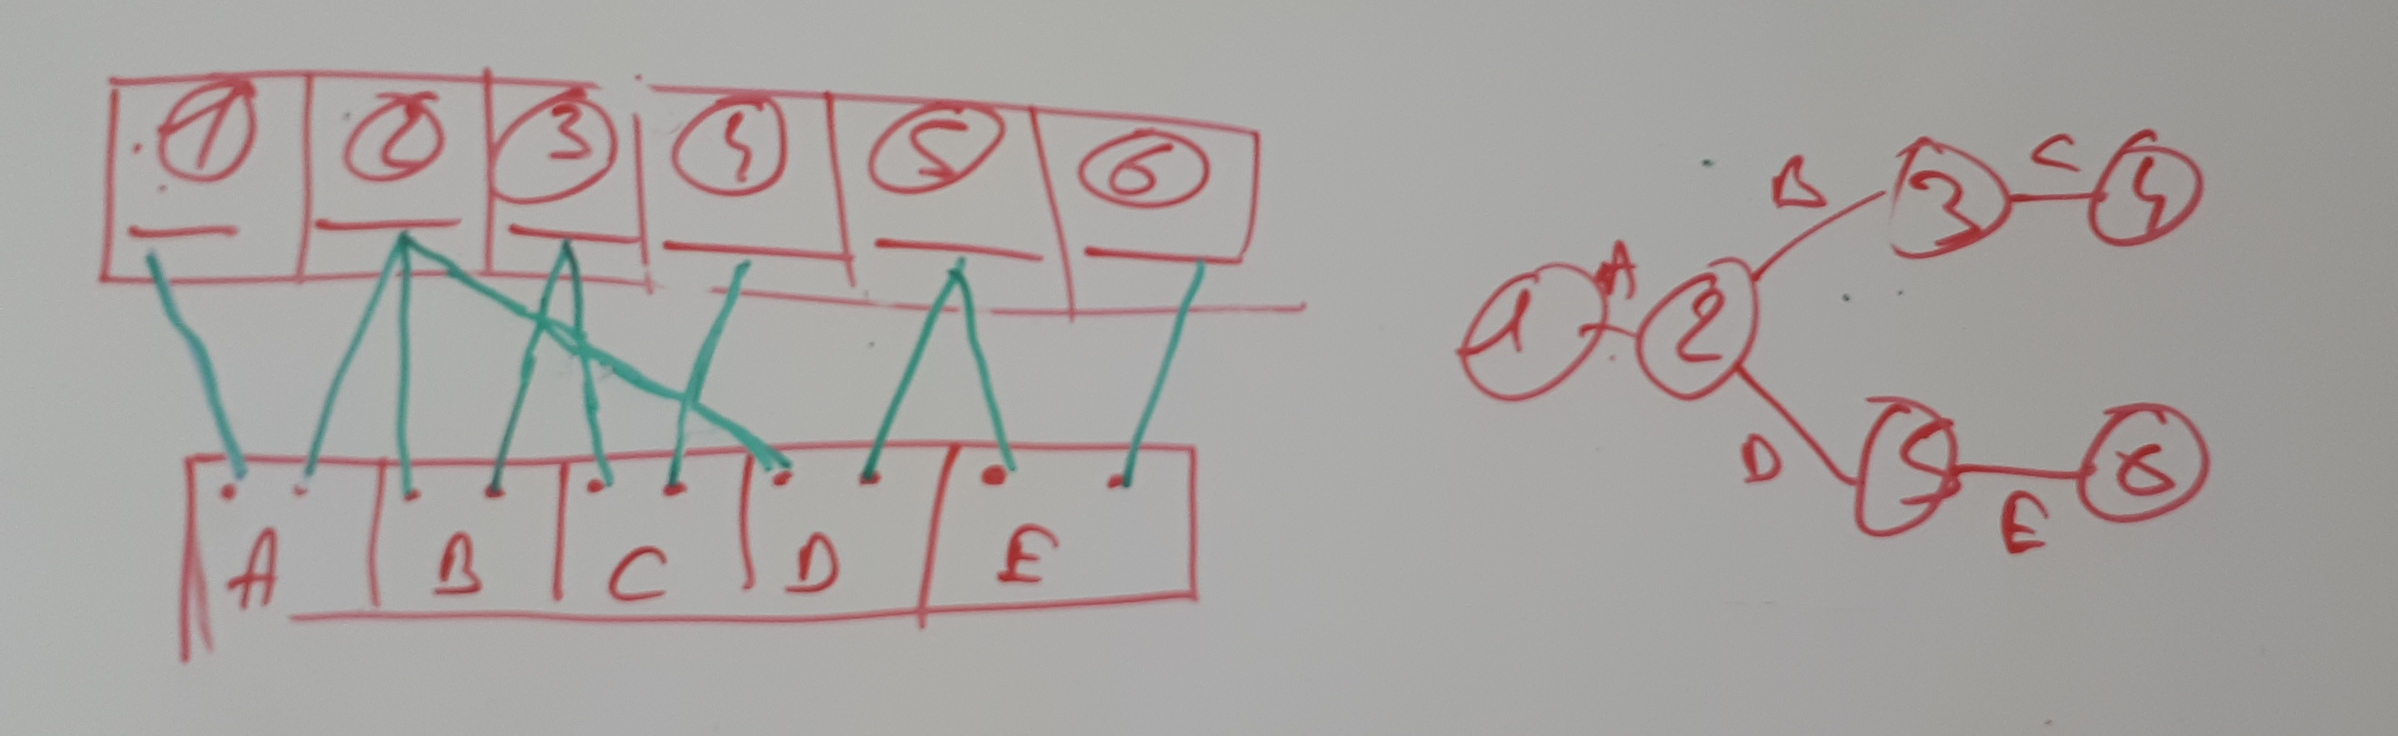
\includegraphics[width=\textwidth]{img/representation_graphe}
	\caption{Représentation du graphe en mémoire}
	\label{fig:representation_graphe}
\end{figure}

\subsection{Données des nœuds et des segments}

Le réseau de dislocations est composé de 2 conteneurs chargés de stocker les informations sur les nœuds et les segments. Bien que la figure \ref{fig:representation_graphe} utilise une représentation Array of Structures, la disposition réelle des données en mémoire reste libre. 

Les conteneurs utilisés doivent pouvoir être parcourus de manière efficace, mais ils doivent aussi s'étendre de manière dynamique. \footnote{thèse A.Etcheverry} s'intéresse à ces conteneurs pour les données dynamiques et évoque 3 types de conteneurs (fig \ref{fig:conteneurs_dynamiques}):
\begin{itemize}
	\item Les tableaux contigus : Le parcours est efficace, mais l'ajout d'objets peut nécessiter une copie des données, et la suppression fragmente la mémoire.
	\item Les listes chainées : L'ajout d'objets ne nécessite pas de ré-allocation, mais le parcours est inefficace
	\item Une \textit{BlockList} : Un conteneur hybride constitué que liste chainée de blocks de données.
\end{itemize}

\begin{figure}
    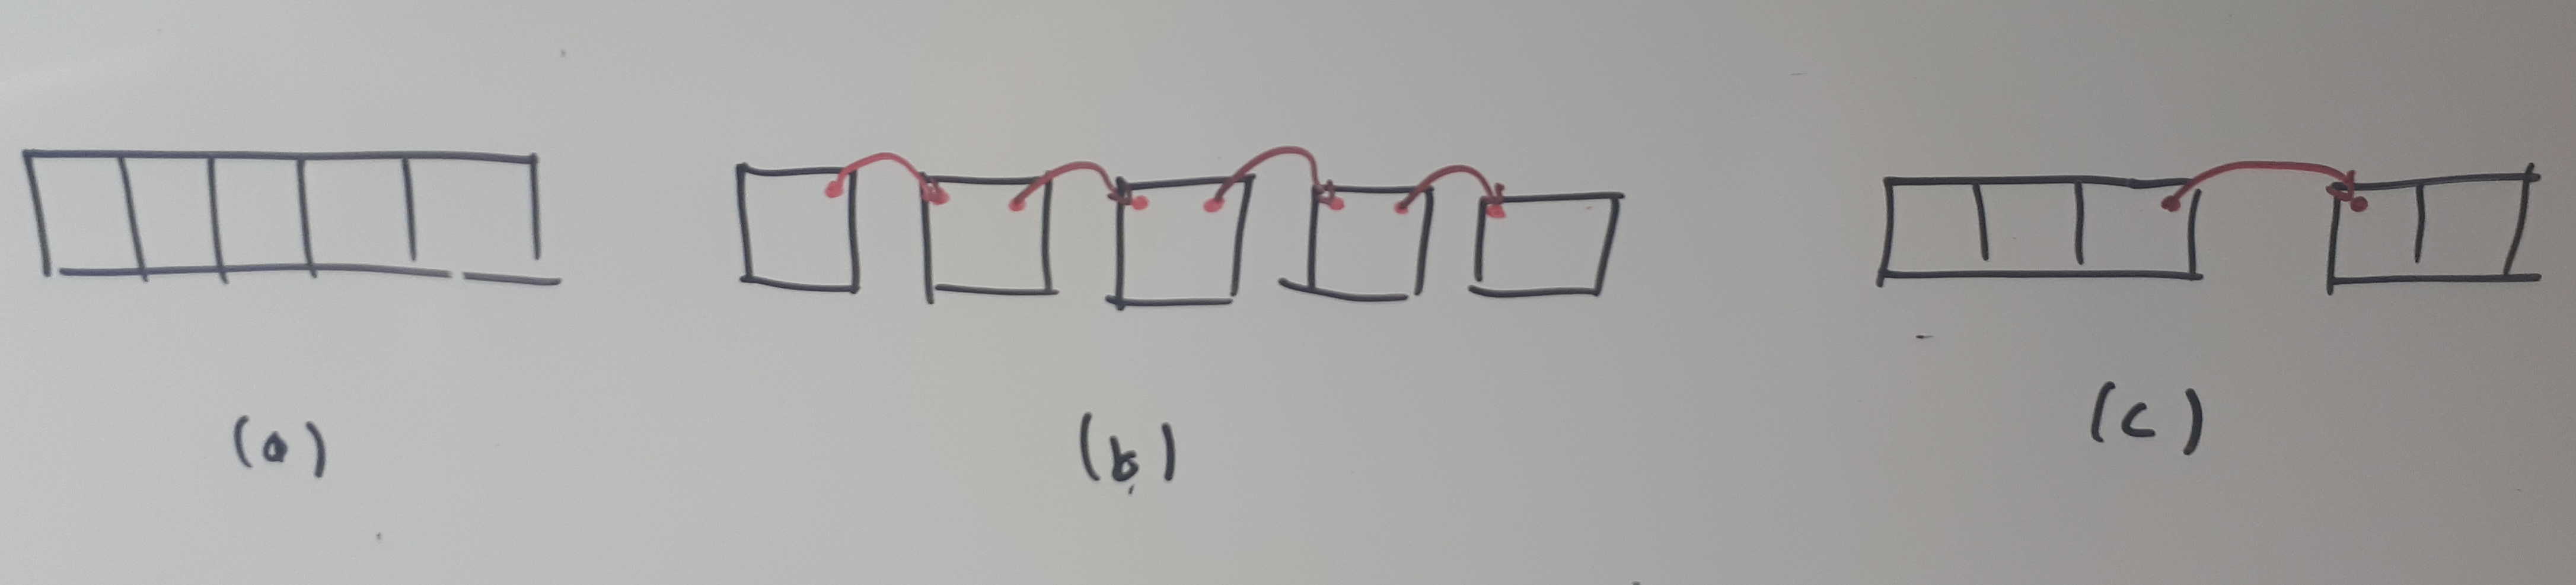
\includegraphics[width=\textwidth]{img/conteneurs_dynamiques}
    \caption{3 types de conteneurs pour données dynamiques.}
    \label{fig:conteneurs_dynamiques}
\end{figure}


Deux implémentations ont été testées. Une implémentation à base de BlockList utilise le code existant de A.Etcheverry détaillé dans sa thèse. Une seconde implémentation utilise des tableaux simples, c'est cette dernière que nous détaillons ici. L'implémentation à base de tableaux utilise des \texttt{std::vector} pour stocker les données concernant les nœuds et les segments. Les interfaces abstraites d'accès aux données que représentent \verb|NodeInfo_ref| et \verb|SegmentInfo_ref| permettent de changer le layout mémoire sans avoir à changer les algorithmes qui accèdent aux données. 

\subsubsection{Soa vs AoS}

Les layouts mémoire classiques sont les suivants:
\begin{itemize}
	\item Array of structures : toutes les informations relatives à un objet sont stockées proche en mémoire, comme l'illustre la Figure \ref{fig:array_of_structures}
	\item Structure of Array (SoA) : chaque donnée possède un tableau indépendant, comme l'illustre la Figure \ref{fig:structure_of_arrays}
\end{itemize}

\begin{figure}[H]
	\centering
	\begin{subfigure}{0.48\textwidth}
		\centering
		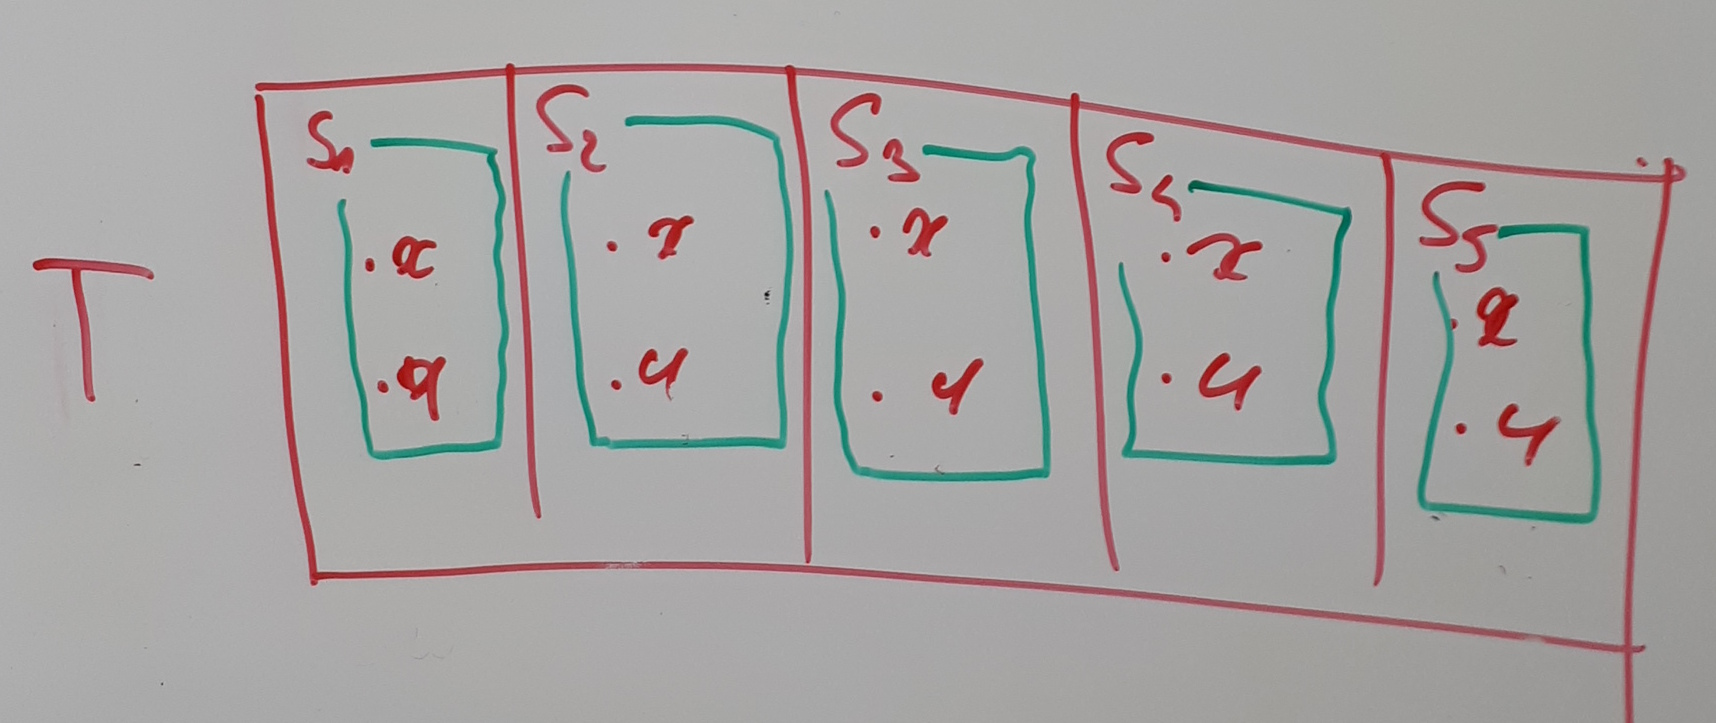
\includegraphics[height=80pt]{img/array_of_structures}
		\caption{Array of Structures}
		\label{fig:array_of_structures}
	\end{subfigure}
	\begin{subfigure}{0.48\textwidth}
		\centering
		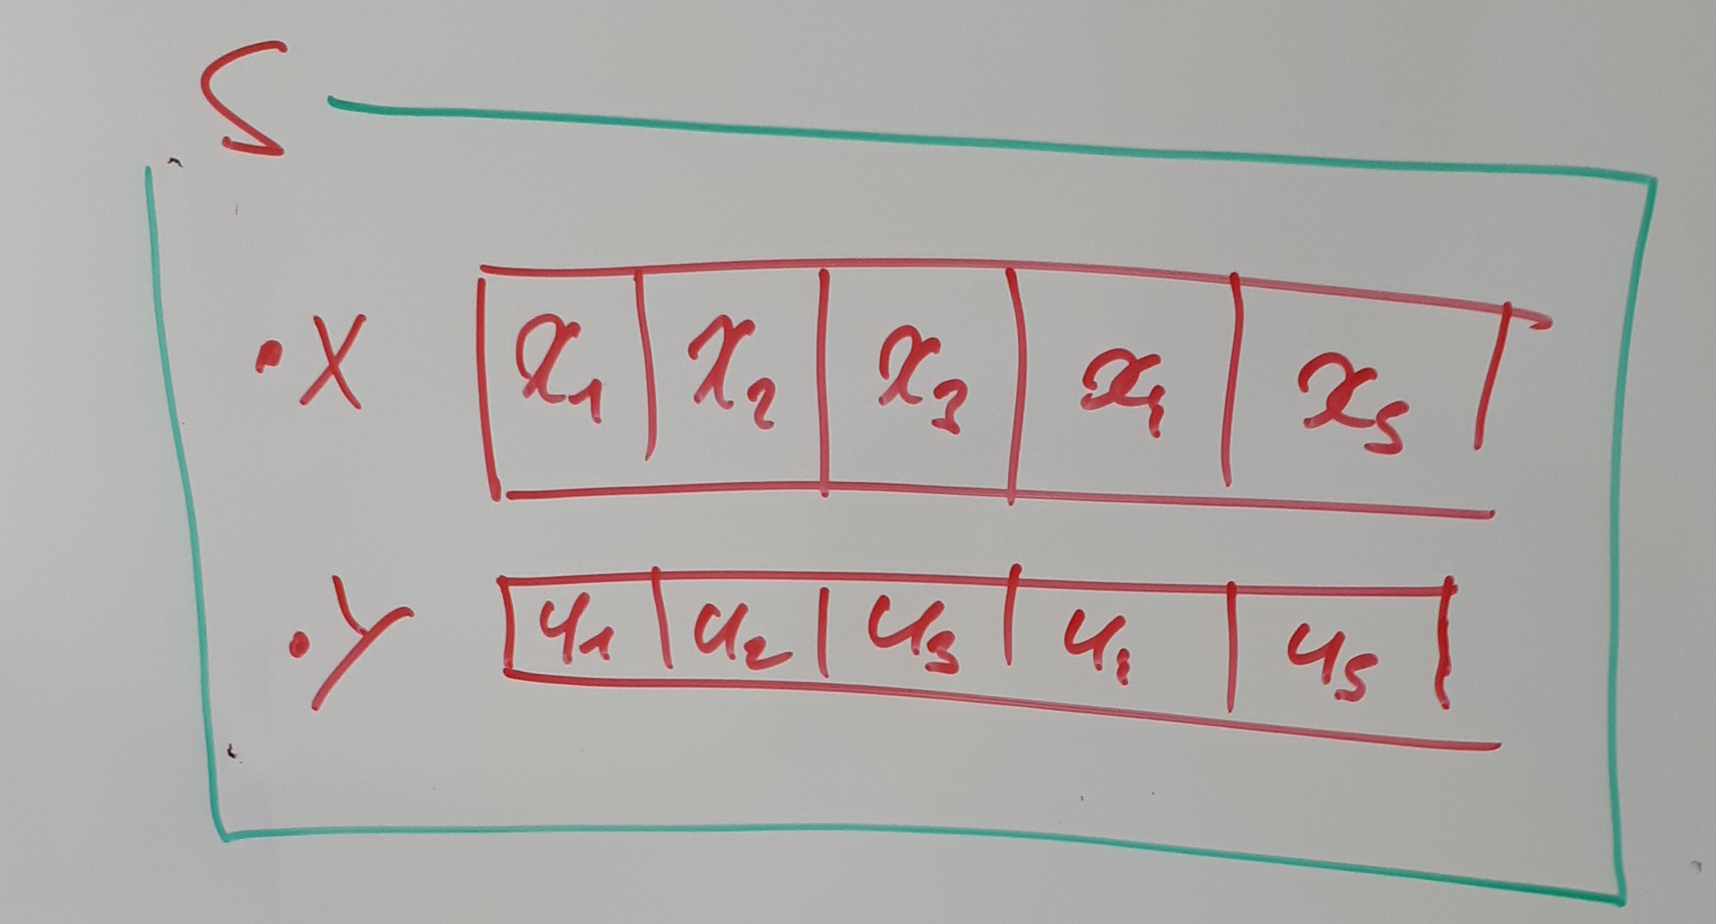
\includegraphics[height=80pt]{img/structure_of_arrays}
		\caption{Structure of Arrays}
		\label{fig:structure_of_arrays}
	\end{subfigure}	
\end{figure}

Dans notre cas le layout Structure of Array est plus approprié car on accède rarement à tous les champs de la structure. Par exemple, pour le calcul des vitesses, on lit les forces et écrit les vitesses en ignorant totalement les positions. AoS nécessite de charger en cache tous les champs, alors que SoA permet de ne charger que les champs utilisés.

\subsubsection{Allocation mémoire}

Le caractère dynamique du réseau de dislocations pousse à ajouter et supprimer fréquemment des objets des conteneurs. 

L'ajout d'objets pose des problèmes lors de l'utilisation de \verb|std::vector| car lorsque l'espace alloué n'est plus suffisant pour ajouter, il faut ré-allouer un buffer et copier les données existantes. Plusieurs solutions existent pour diminuer l'impact de ce problème :
\begin{itemize}
	\item \verb|std::vector| amorti le cout de d'insertion en augmentant la taille de son buffer de manière géométrique (ex : le nouveau buffer et 2x plus grand que le précédent)
	\item Lorsque la taille finale est connue ou bornée, il est possible d'allouer un buffer de taille suffisante avec \verb|std::vector::reserve()|
\end{itemize}
En pratique, dans Optidis, pour régler ce problème, il faut utiliser \verb|std::vector::reserve()| lorsque l'on initialise le réseau de dislocations, et on utilise par la suite le cout constant amorti de l'insertion dans \verb|std::vector|. Une insertion qui déclenche une ré-allocation aura un cout important, mais ne devrait pas arriver de manière trop fréquente.

\subsubsection{Fragmentation mémoire}
\label{sec:fragmentation_memoire}

Les suppressions/ajouts d'objets dans le réseau de dislocations pose des problèmes de fragmentation mémoire en laissant des "trous" dans la structure de données. Plusieurs solutions existent pour limiter la fragmentation.

\paragraph{Nettoyage périodique}
La première solution (Figure \ref{fig:fragmentation_memoire}a) consiste à insérer les nouveaux éléments à la fin du buffer mémoire, et invalider les éléments supprimés. La structure peut être nettoyée périodiquement. Cette solution peut poser un problème d'efficacité mémoire selon la fréquence de nettoyage de la structure. De plus, les objets ne sont pas contigus en mémoire, et il faut faire un test pour savoir si l'élément est invalidé ou non au cours du parcours.

\paragraph{Remplissage à l'insertion}
La seconde solution (Figure \ref{fig:fragmentation_memoire}b) consiste à réinsérer les nouveaux éléments à la place des éléments supprimés. Cependant, certains algorithmes stockent des indices sur des objets supprimés, et cela pose un problème si l'objet à été remplacé.

\paragraph{Remplissage à la suppression}
La troisième solution (Figure \ref{fig:fragmentation_memoire}c) consiste à remplacer les éléments supprimés dès leur suppression par un autre élément se trouvant en fin de zone mémoire. Cela pose un problème, car on invalide alors tout iterateur vers le dernier élément du tableau. Il faudrait alors mettre à jour la topologie dans chaque nœud/segment.

\begin{figure}[H]
	\centering
		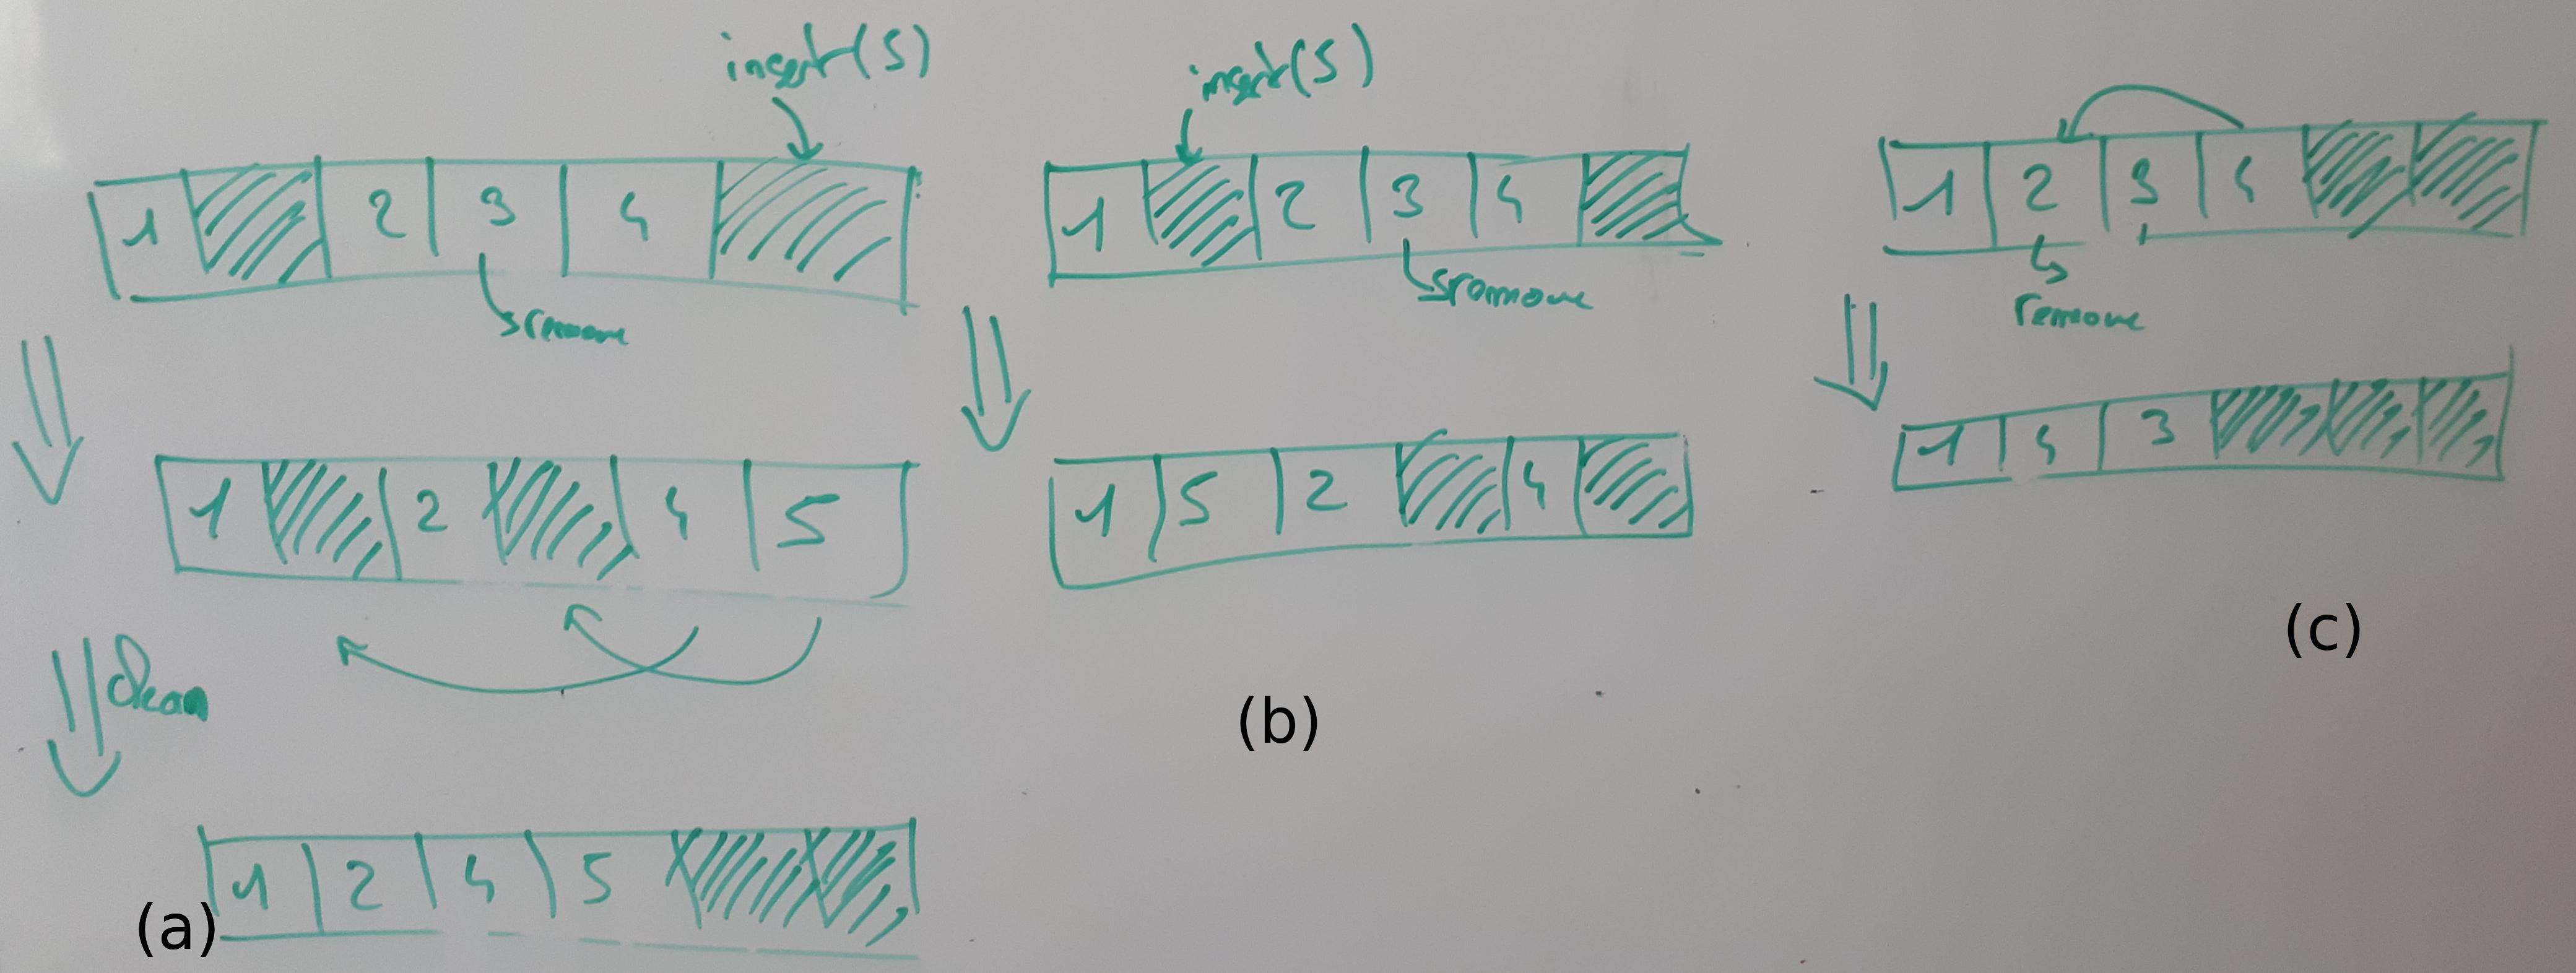
\includegraphics[width=\textwidth]{img/fragmentation_memoire}
		\caption{Solutions à la fragmentation mémoire}
		\label{fig:fragmentation_memoire}
\end{figure}


\subsection{Données distribuées avec MPI}

La structure de données prévoit une interface compatible avec les données distribuées, comme indiqué en section \ref{sec:TAD-distribué}. Cette section explique de quelle manière les données sont distribuées, et comment sont implémentées les opérations collectives.

\subsubsection{Décomposition de domaine}

Les données sont distribuées selon une décomposition de domaine suivant la courbe de Morton pour une compatibilité avec ScalFMM. L'espace est découpé en boites selon une grille uniforme qui sont distribuées sur les différents processus MPI. Les boites sont ordonnées selon la z-curve, et des intervalles de boites sont associés aux différents processus MPI, comme l'illustre la figure \ref{fig:domaindecomposition_morton_interval}.

\begin{figure}[]
    \centering
    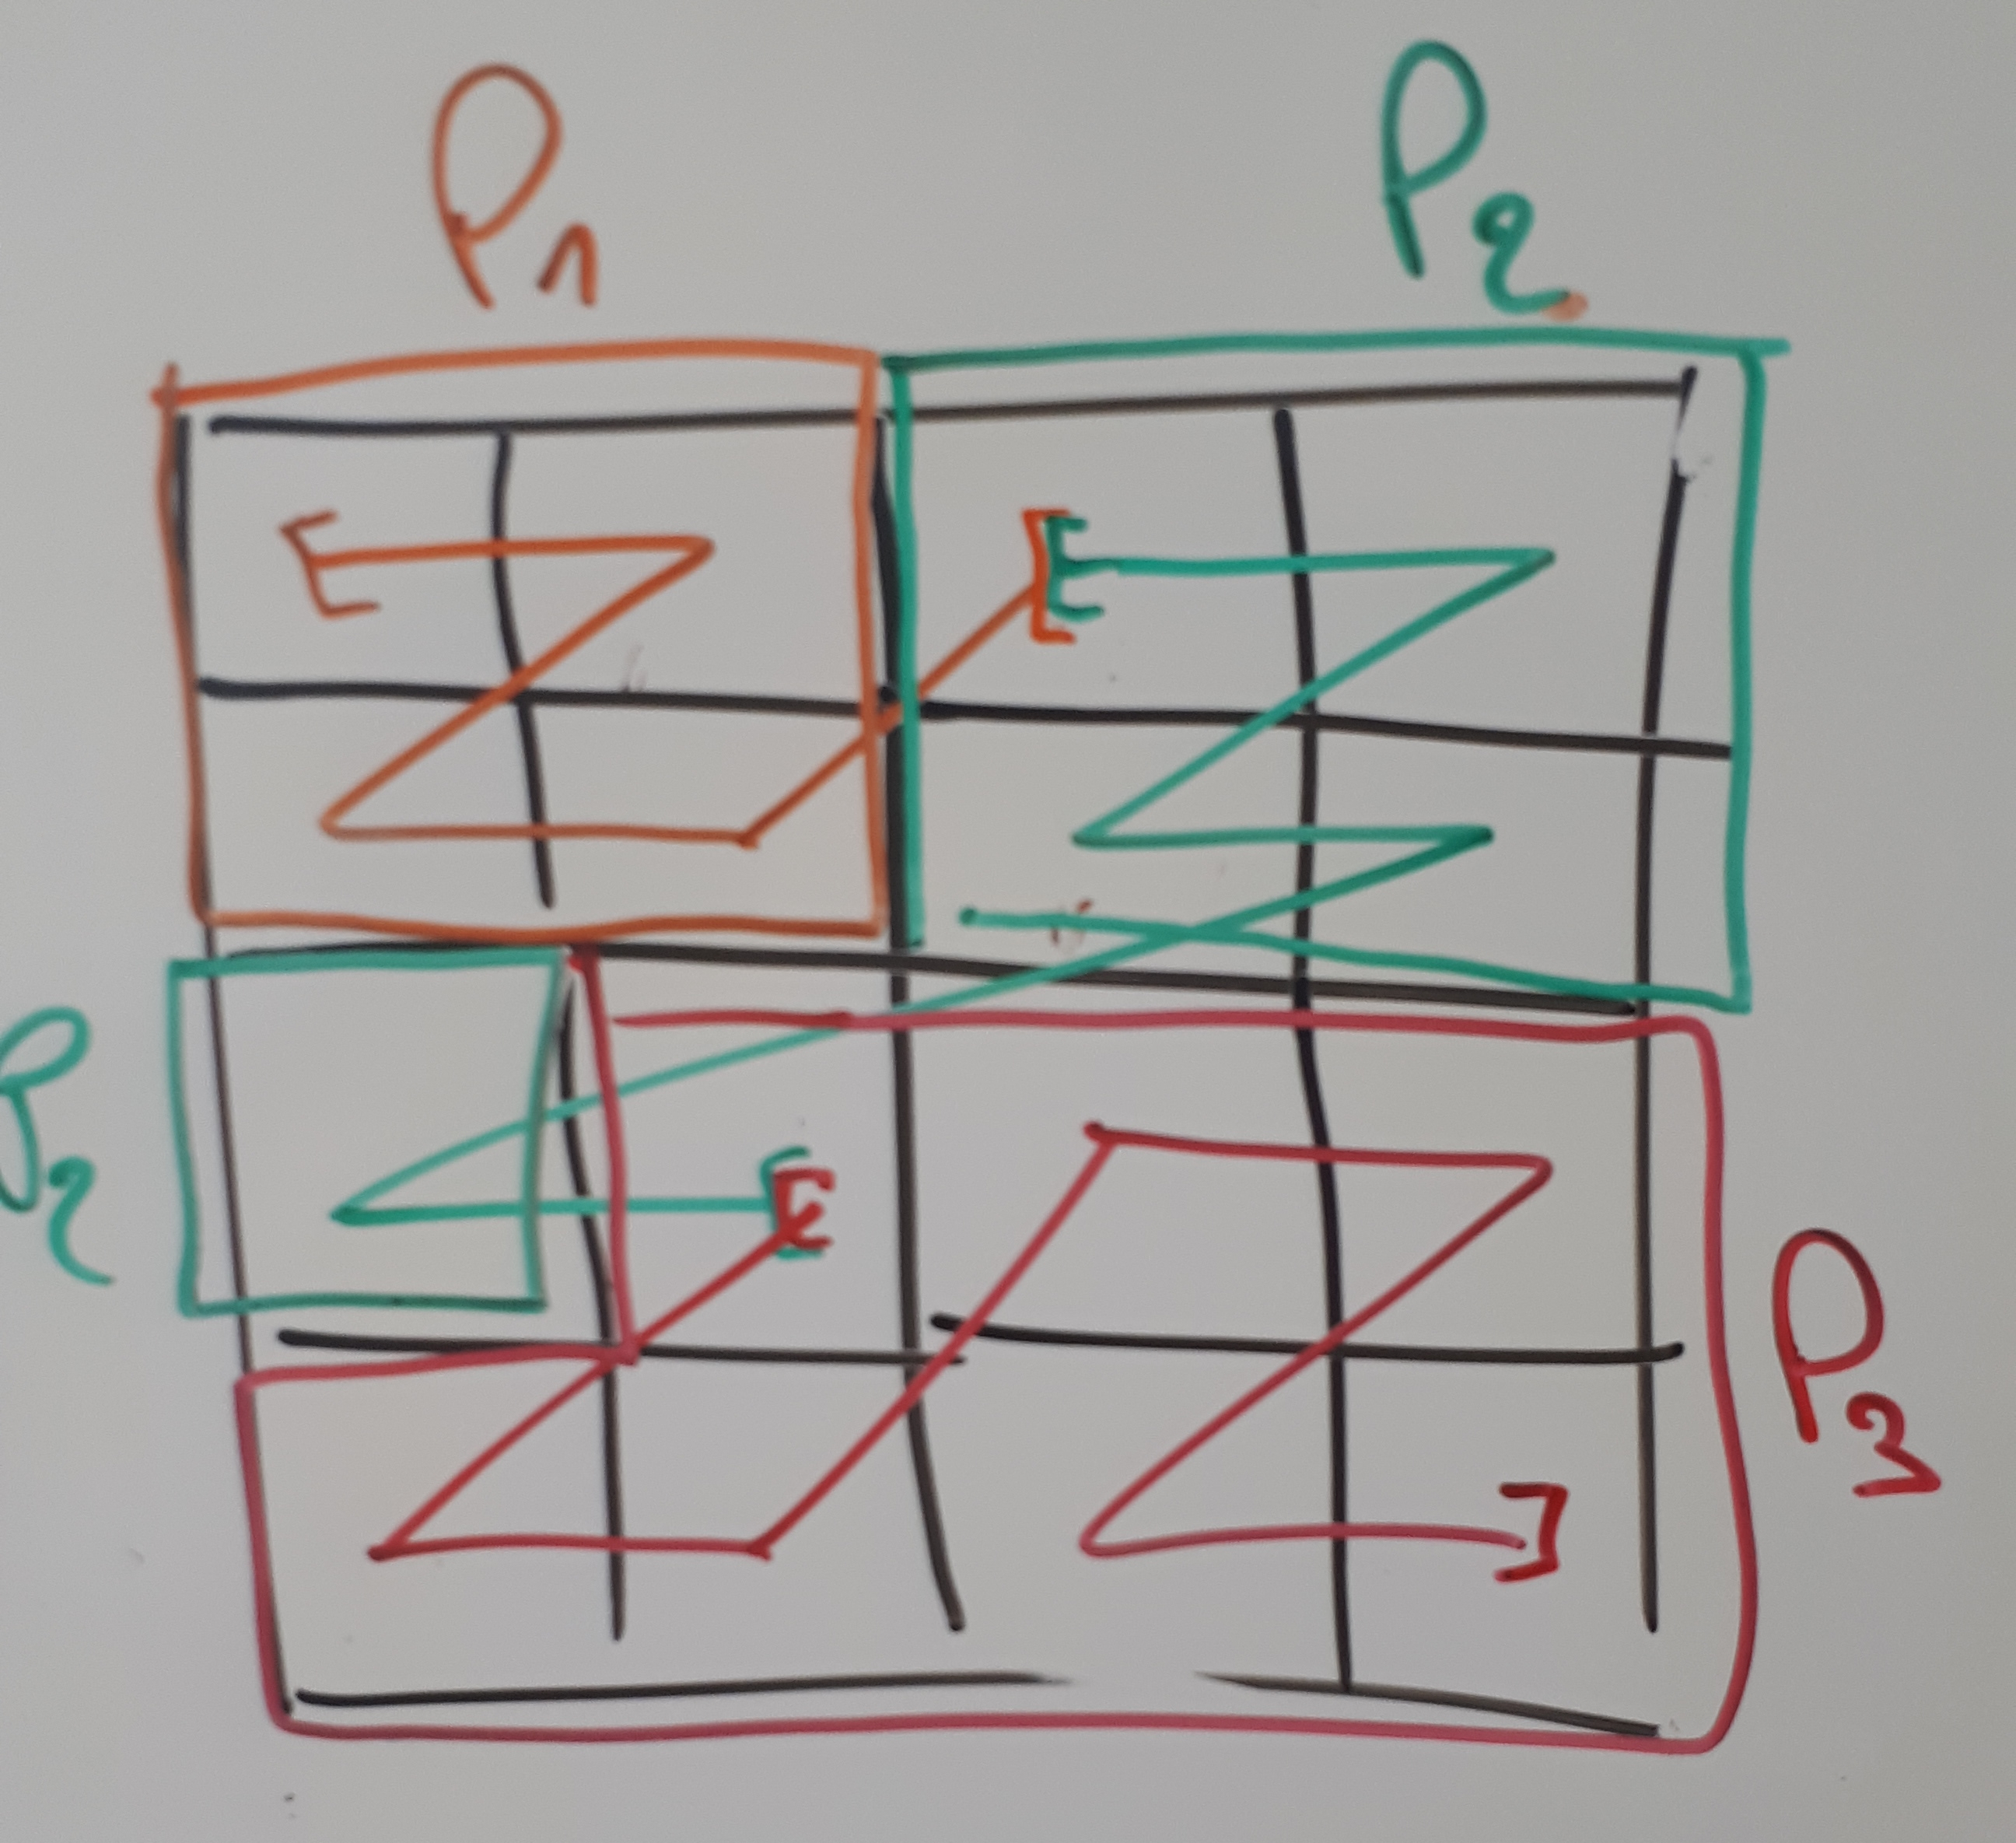
\includegraphics[width=0.5\textwidth]{img/domaindecomposition_morton_interval}
    \caption{Décomposition de domaine par intervalles de Morton}
    \label{fig:domaindecomposition_morton_interval}
\end{figure}

Pour distribuer les objets sur les processus MPI, on utilise les règles suivantes issues de \footnote{thèse aetchev}:
\begin{itemize}
    \item L'indice de Morton associé à un nœud $\mathcal{M}(n)$ est l'indice de Morton de la boite ou il se trouve
    \item L'indice de Morton associé à un segment $\mathcal{M}(s)$ est l'indice de Morton de la boite ou se trouve son centre
    \item Chaque processus $P_i$ se voit attribué des intervalles $I_{P_i}$ d'indices de Morton formant une partition du domaine
    \item Chaque objet $o$ (segment ou nœud) est associé au processus $P_i$ unique dont l'intervalle contient son indice de Morton:
\end{itemize}

\begin{equation}
    o \in P_i \Leftrightarrow \mathcal{M}(o) \in I_{P_i}
\end{equation}

Pour que la décomposition de domaine soit compatible avec ScalFMM, il faut s'assurer que toutes les particules d'une feuille de l'octree FMM se trouvent sur le même processus MPI. La décomposition de domaine doit se faire selon les boites d'un octree d'une hauteur inférieure à l'arbre utilisé pour le calcul FMM, comme l'illustre la figure \ref{fig:domaindecomposition_smaller_octree}a, sinon certaines boites FMM seront éclatées sur plusieurs processus, comme dans la figure \ref{fig:domaindecomposition_smaller_octree}b.

\begin{figure}[]
\centering
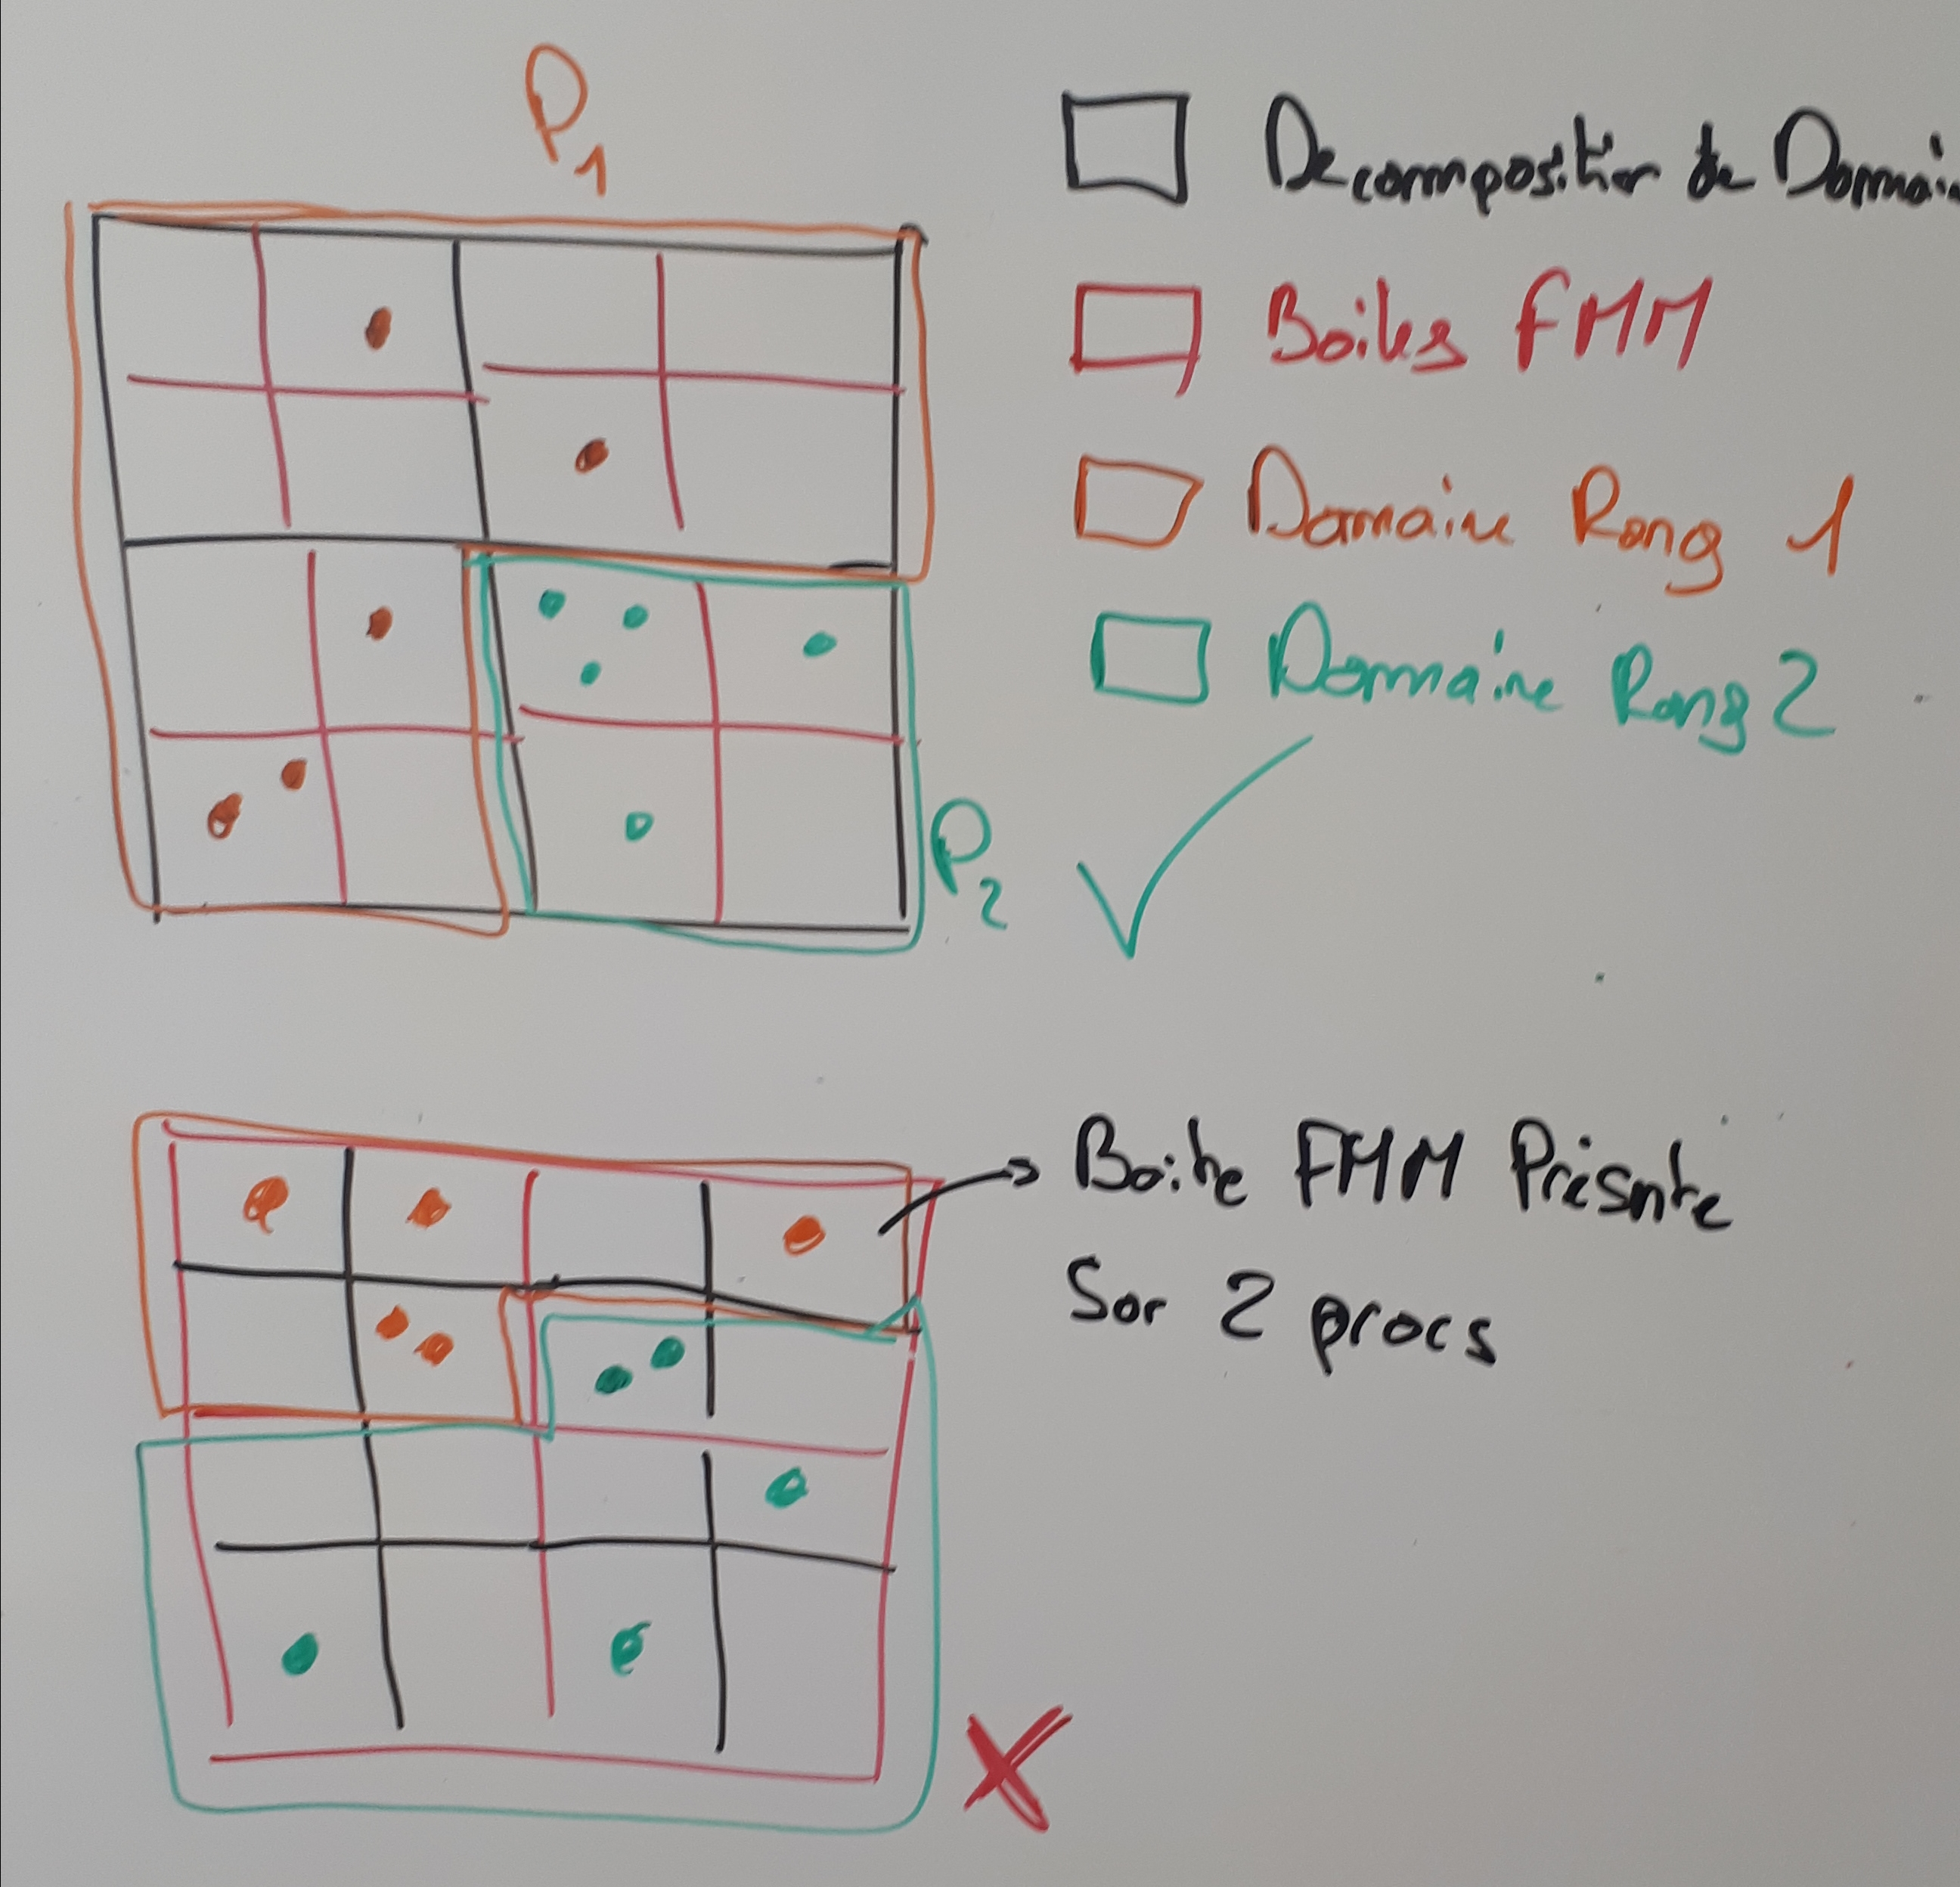
\includegraphics[width=0.5\textwidth]{img/domaindecomposition_smaller_octree}
\caption{Compatibilité de la décomposition de domaine avec ScalFMM}
\label{fig:domaindecomposition_smaller_octree}
\end{figure}

\subsubsection{Équilibrage de charge}

La charge peut être équilibrée en ajustant les intervalles de chaque processus. La métrique choisie pour l'équilibrage de charge est le nombre d'objets par processus : pour une charge équilibrée, chaque processus doit avoir autant de nœuds et de segments. Pour déterminer les intervalles optimaux plusieurs approches sont possibles : \footnote{thèse aetchev} propose une approche dynamique basée sur la communication avec les voisins, \footnote{Fast Sorting on a Distributed-Memory Architecture - Cheng, Shah} propose une approche basée sur un algorithme de k-sélection parallèle. L'approche choisie se déroule en deux étapes, sur le modèle de \footnote{Fast Sorting on a Distributed-Memory Architecture - Cheng, Shah} :

Une première étape détermine les intervalles optimaux un utilisant un algorithme de sélection sur la liste des indices de Morton des particules. Le $k_i^{eme}$ plus petit indice de Morton des objets marquera le début de l'intervalle $I_{P_i}$ avec : 
\begin{equation}
    k_i=\frac{i \cdot size}{nb_{procs}}
\end{equation}

Deux algorithmes de sélection ont été testés pour déterminer ces intervalles : 
\begin{itemize}
	\item Un algorithme séquentiel : la lise des indices de Morton est rassemblée sur un unique processus qui se chargera de les trier, et de sélectionner les $k_i$;
	\item Un algorithme parallèle : Chaque processus trie sa liste d'indices de Morton et communique avec les autres pour déterminer les $k_i$ sur le modèle de  \footnote{Fast Sorting on a Distributed-Memory Architecture - Cheng, Shah}. 
\end{itemize}

La seconde étape consiste en une migration des objets vers les nouveaux intervalles détaillé en section \ref{sec:migration}.

\subsubsection{Migration}

Après avoir déplacé les objets dans la phase d'intégration ou après avoir modifié les intervalles de décomposition de domaine dans la phase de load balancing, certains objets peuvent se trouver dans des boites qui appartiennent à un autre processus MPI. La phase de migration déplace les objets vers les bons processus MPI. 

La migration contourne l'interface d'insertion/suppression évoquée en section \ref{} pour des raisons de performances. L'implémentation de cet algorithme doit donc mettre à jour les informations internes de la structure de données qui sont normalement maintenues en cohérence par les opérations collectives d'ajout/suppression.

La migration se déroule en plusieurs phases:
\begin{itemize}
	\item Un parcours sur les objets est effectué pour déterminer quels objets doivent être déplacés sur quels domaines. Les objets à déplacer sont supprimés des listes locales.
	\item Les processus échangent les objets (alltoall)
	\item Les objets reçus sont insérés dans ls listes locales.
	\item Les informations internes à la structure de données, comme la topologie, sont mises à jour. Par exemple, les indices des segments connectés aux nœuds sont mis à jour avec les nouveaux indices des segments déplacés.
\end{itemize}


\subsubsection{Parcours}

Certaines fonctions de parcours nécessitent d'effectuer des communications, comme par exemple le parcours des nœuds avec leur voisinage.

Pour optimiser les communications, la structure de données peut maintenir une liste des indices des nœuds connectés à des segments distants, et des segments connectés à des nœuds distants. Chaque processus MPI sait alors quels objets doivent être envoyés avant le parcours, et peut initier les communications avant d'itérer sur les objets locaux. Le parcours s'effectue en deux phases : le parcours des objets locaux, puis le parcours des objets connectés à des objets distants. Les liste des objets à communiquer sont maintenues lors des opérations d'ajout et de suppressions d'objets dans le réseau de dislocation.

Parmi les améliorations possibles des communications MPI :
\begin{itemize}
\item Recouvrir les communications par le calcul en itérant sur les objets locaux pendant la communication.
\item Améliorer la liste des objets à envoyer en ajoutant pour chaque objet la destination.
\end{itemize}

\subsubsection{Nettoyage}

La structure de données doit être nettoyée périodiquement afin d'éviter la fragmentation mémoire, comme l'évoque la section \ref{sec:fragmentation_memoire}. Ce nettoyage à pour but de remplir les "trous" dans la structure de données. 

Comme pour la migration, le nettoyage de la structure de données contourne l'interface d'ajout/suppression des objets, il faut donc faire attention à maintenir en cohérence les informations internes à la structure.

La solution choisie consiste en un tri des objets selon leur indice de Morton et supprimant les objets invalidés. Cette solution permet de maintenir la cohérence spatiale des objets en plus de supprimer les "trous" dans la structure. Le tri s'effectue en deux étapes comme le montre la figure \ref{fig:nettoyage_tri}
\newcommand*\circled[1]{\tikz[baseline=(char.base)]{ \node[shape=circle,draw,inner sep=1pt] (char) {#1};} }
\begin{itemize}
	\item \circled{1} Une permutation est générée en triant les indices de Morton;
	\item \circled{2} tous les objets sont copiés dans une nouvelle liste triée en utilisant la permutation.
\end{itemize}
Cela permet de séparer l'étape de tri en $O(nlog(n))$ de l'étape de copie des objets qui peut bénéficier de certaines optimisations et du parallélisme.

\begin{figure}
	\centering
	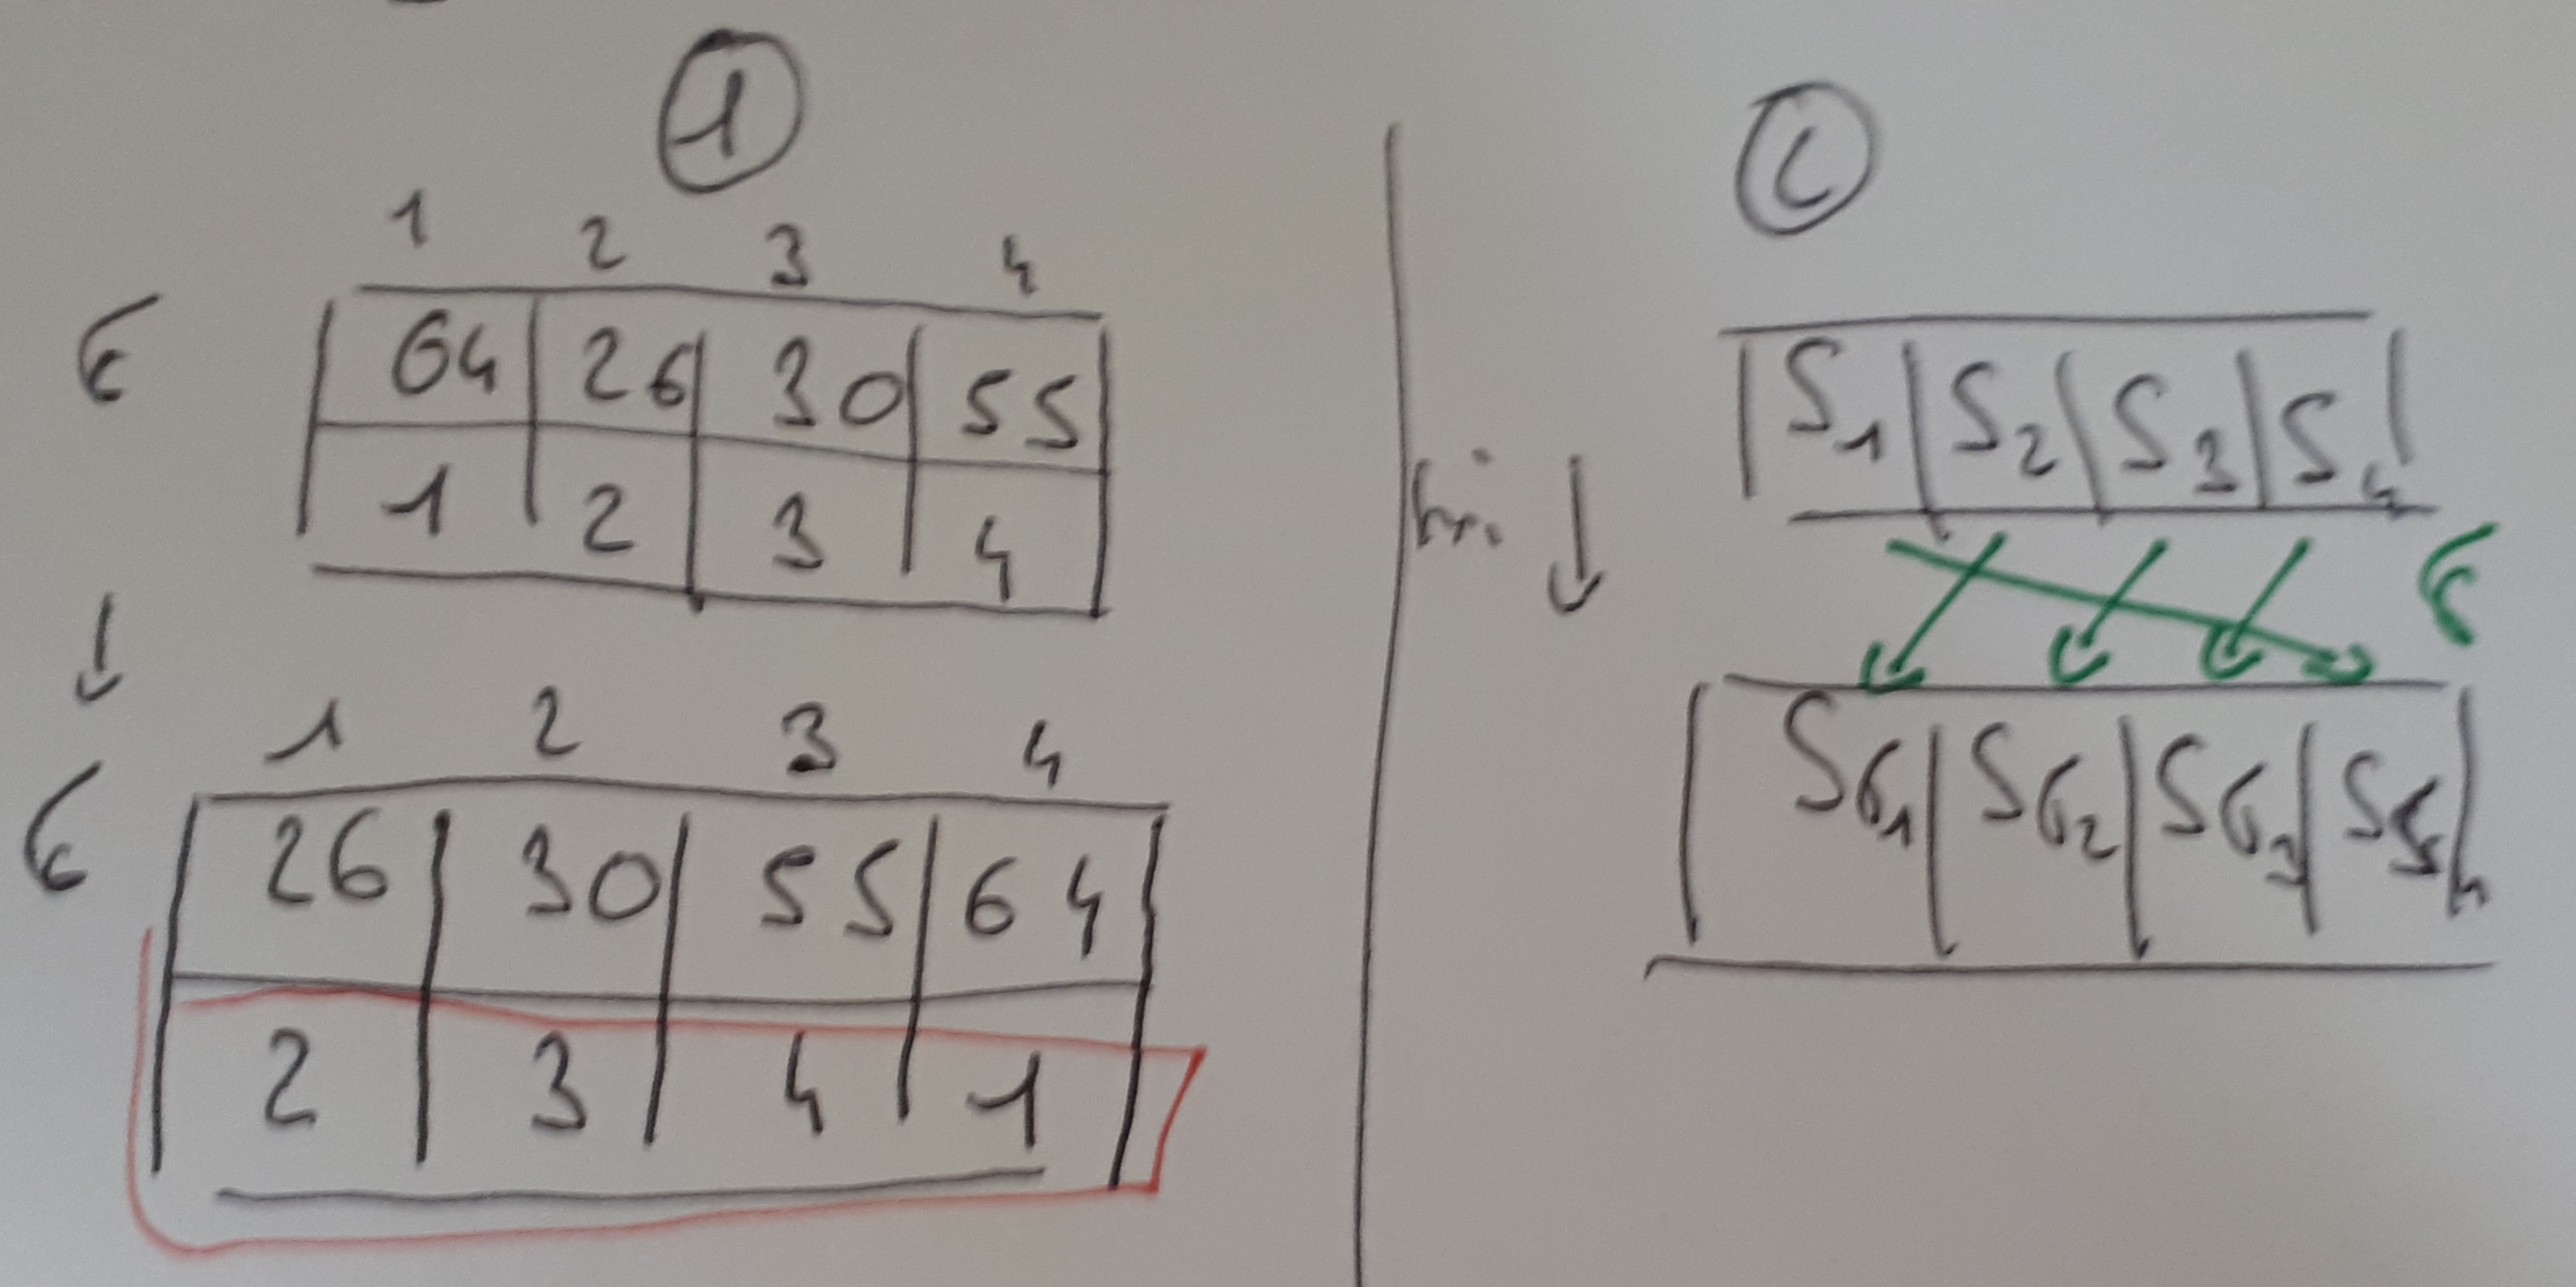
\includegraphics[width=0.5\textwidth]{img/nettoyage_tri}
	\caption{Tri des objets lors de la défragmentation}
	\label{fig:nettoyage_tri}
\end{figure}

La permutation est générée en utilisant \verb|std::sort()| sur un tableau $\sigma$ contenant des paires $\{morton, indice\}$. $\sigma$ est initialisé par en utilisant l'indice de morton du $i_{ème}$ objet, et la position courante de l'objet : 

\begin{equation}
\sigma_i \leftarrow \{m_i, i\}
\end{equation}

Pour les objets supprimés, on utilise $+\infty$ comme indice de Morton, de manière à ce que les objets supprimés soient déplacés en fin de tableau. Une fois le tableau $\sigma$ trié selon les indices de Morton, l'indice contenu dans chaque paire donne la permutation $\sigma(i)$ qu'il faut appliquer pour que les objets soient triés. Il ne reste plus qu'à les copier dans une nouvelle liste en respectant cette permutation :

\begin{equation}
new\_objects[i] \leftarrow old\_objects[\sigma(i)]
\end{equation}




\subsection{Multithreading avec OpenMP}

Les parcours de la structure de données décrits en section \ref{sec:TAD-algos_parcours}, ainsi que les itérateurs supportent le multithreading avec OpenMP. 

\subsubsection{itérateurs}

Les itérateurs utilisent OpenMP pour calculer les indices de début et de fin pour chaque thread d'une région parallèle. Par exemple, pour parcourir les nœuds en parallèle, il suffit de mettre la boucle dans une région parallèle\footnote{L'exemple utilise les \textit{Range-based for loops} du C++11 qui utilisent les itérateurs et les méthodes begin() et end()}:

\begin{minted}{cpp}
    #pragma omp parallel
    for(Mesh::NodeInfo_ref n : mesh.nodes)
    {
        f( n );
    }
\end{minted}

Les méthodes begin() et end() retournent sur chaque thread un intervalle, et l'ensemble des intervalles de tous les threads forme une partition. Dans notre implémentation, chaque thread i parcourt les éléments valides de l'intervalle $[B_i, B_{i+1}]$ du conteneur de taille $size$ qui stocke les nœuds ou les segments.

\begin{equation}
    B_i = \left \lfloor{\frac{i \cdot size}{nb_{threads}}}\right \rfloor 
\end{equation}

L'utilisation des itérateurs permet le parcours des données de manière indépendante de l'implémentation, mais la performance n'est pas optimale avec cette interface.

\subsubsection{Fonctions de parcours}

Les fonctions de parcours présentées en section \ref{sec:TAD-algos_parcours} sont aussi compatibles avec OpenMP. Une implémentation basique utilise les itérateurs du paragraphe précédent pour parcourir les données. Il faut porter une attention particulière aux communications MPI qui doivent se dérouler sur un seul thread.

Les fonctions de parcours peuvent être implémentées spécifiquement pour une implémentation de la structure de donnée en cassant l'encapsulation. Cela permet d'utiliser les spécificités d'une implémentation pour écrire un parcours plus efficace.

Des fonctions de parcours spécifiques ont été implémentées pour l'implémentation de \verb|Mesh| utilisant des \verb|std::vector|, et permettent de meilleures performances. Elles utilisent la directive \verb|#pragma omp for| pour paralléliser avec OpenMP, et accèdent directement aux \verb|std::vector| pour des indirections plus efficaces.
